\documentclass[10pt,a4paper]{article}
\usepackage{tabularray}
\usepackage{tikz}             
\usepackage{xeCJK}
\usepackage{amsthm}  
\usepackage[fontset=macnew]{ctex}
\usepackage{sgame}
\usepackage{geometry}
\usepackage{amsmath}
\usepackage{amssymb}
\usepackage{graphicx}
\usepackage{sectsty}
\usepackage{color}
\geometry{left=2.cm,right=2.cm,top=3.18cm,bottom=3.18cm}
\usepackage{pgfplots} % package used to implement the plot
\usepackage{pgf-pie}
\usepackage{exscale}
\usepackage{relsize}
\pgfplotsset{width=6.5cm, compat=1.6}
\usepackage{indentfirst}
\usepackage{float}
\usetikzlibrary{shapes,arrows}
\sectionfont{\color{blue}\selectfont}
\subsectionfont{\color{blue}\selectfont}
\subsubsectionfont{\color{blue}\selectfont}
\usepackage{hyperref}
\usepackage{marvosym}
\usepackage{color}
\usepackage{minted}
\usemintedstyle{xcode}
\usepackage{memorygraphs}
\usetikzlibrary{calc,shapes.multipart,chains,arrows.meta}
\usepackage{caption}
\usepackage{makecell}
\newtheorem{definition}{定义}
\newtheorem{theorem}{\textcolor{red}{定理}}
\newtheorem*{solution}{\kaishu 解}
\usepackage[skins]{tcolorbox} %必须标注skin,才能使用shadow命令显示阴影。
\tcbuselibrary{breakable} %breakable:支持跨页
\usepackage{fancyhdr} % 导入fancyhdr包
\pagestyle{fancy}
% 页眉设置
\fancyhead[L]{\textbf{龚舒凯\ 2022202790}}

\begin{document}
	\title{{\Huge 数据结构与算法I实验报告{\large\linebreak\\}}{\huge 实验2:区块链(1)\linebreak\linebreak}}
	\vspace{3cm}
	%\author{\Large 龚舒凯\ 2022202790\ 应用经济-数据科学实验班}
	\author{\\ \Large 龚舒凯\ 2022202790\ 应用经济-数据科学实验班\\
		\hfill\\
		\Large{\url{https://github.com/GONGSHUKAI}}\\
		\hfill}
	
	\date{\today}
	\maketitle
	\newpage
	\begin{center}
		{\huge \textbf{区块链(1)}}
	\end{center}
	\section{需求分析}
    \noindent \textbf{问题描述:}区块链,就是一组区块构成的“链”,也就是链表。下面关于区块和交易的定义来自比特币系统,根据任务需要作了简化。在比特币系统中,采用的是UTXO模型,即每个交易将使用前面某个交易的输出(output)来作为当前交易的输入(input)。而当前交易的输出将作为未来某个交易的输入。
    \begin{figure}[htbp]
		\centering
		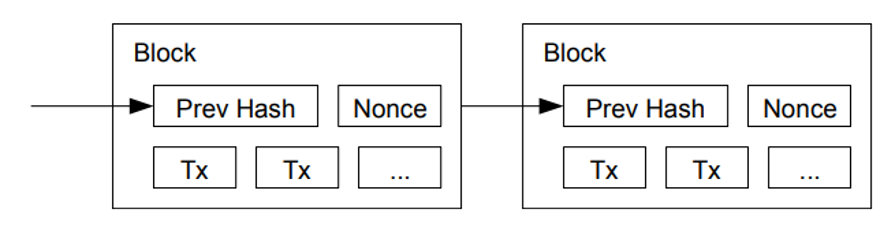
\includegraphics[width=0.7\linewidth]{BlockChainTransactions.png}
		\caption{区块链示意图}	
	\end{figure}
    区块链中各要素的定义如下:
    \begin{itemize}
        \item \textbf{区块(Block):}区块为区块链中的基本单位,其内涵成员如下:
        \begin{table}[H]
            \centering
            \begin{tabular}{|l|l|l|}
            \hline
                成员名 & 类型 & 说明 \\ \hline
                height & 整数 & 当前块的高度,一条链上每个区块的Height均不相同。 \\ \hline
                hash & 字符串 & 本区块的哈希值。  \\ \hline
                prevHash & 字符串 & 前一个区块的哈希值,本实验中可以置空 \\ \hline
                merkleRoot & 字符串 & 本区块中所有交易的默克尔树根,本实验中可以置空 \\ \hline
                nonce & 整数 & 神秘数,本实验可以忽略  \\ \hline
                transactions & 数组 & 一组交易(transaction)的集合 \\ \hline
            \end{tabular}
        \end{table}
        \item \textbf{交易(Transaction):}
        \begin{table}[H]
            \centering
            \begin{tabular}{|l|l|l|}
            \hline
                成员名 & 类型 & 说明 \\ \hline
                txid & 字符串 & 交易的编号,具有唯一性 \\ \hline
                input\_count & 整数 & inputs的数量,本实验可以忽略 \\ \hline
                output\_count & 整数 & outpus的数量,本实验可以忽略 \\ \hline
                inputs & 数组 & 一组input的集合,表示当前交易的输入所用到的输出 \\ \hline
                outputs & 数组 & 一组output的集合,表示当前交易的输出,可能作为后续交易的输入 \\ \hline
                is\_coinbase & 整数 & 表示是否为coinbase交易(1为coinbase交易,0为非coinbase交易) \\ \hline
            \end{tabular}
        \end{table}
        \item \textbf{输入(Input):}
        \begin{table}[H]
            \centering
            \begin{tabular}{|l|l|l|}
            \hline
                成员名 & 类型 & 说明 \\ \hline
                pre\_block & 整数 & 该input所引用的output所在区块的高度;  \\ \hline
                prevTxID & 整数 & 该input所引用的output所在交易的txID \\ \hline
                prevTxOutIndex & 整数 & 该input所引用的output位于所在交易output集合中的索引 \\ \hline
                scriptSig & 字符串 & 脚本和签名,本实验中可以置空 \\ \hline
            \end{tabular}
        \end{table}
        \item \textbf{输出(Output):}
        \begin{table}[H]
            \centering
            \begin{tabular}{|l|l|l|}
            \hline
                成员名 & 类型 & 说明 \\ \hline
                txid & 字符串 & 该output所属的交易 \\ \hline
                index & 整数 & 该output在所属交易中的索引值 \\ \hline
                value & 整数 & 该output的价值 \\ \hline
                script & 字符串 & 脚本,本实验可以置空 \\ \hline
            \end{tabular}
        \end{table}
    \end{itemize}
    \noindent \textbf{基本要求:}
    \begin{enumerate}
        \item 读入区块相关数据文件demo.zip(包括blocks.csv,transaction.csv,inputs.csv,outputs.csv四个文件),生成区块数据变量,将所有区块按高度顺序组织成链表。
        \item 检验区块链中交易(Transactions)的合法性:根据如下三条规则判断区块中交易合法与否:
        \begin{enumerate}
            \item 每个input所使用的output能够找到。(例外:coinbase$=1$的交易可以没有input,只有output。该类交易是合法的,其中的output可能被后续的transaction所引用。)
            \item 每个input所使用的output没有被之前的交易用过,且引用的output必须来自合法的交易。
            \item 该交易所有input所引用的output的价值(value)之和大于等于该交易所有output的价值(value)之和。
        \end{enumerate}
    \end{enumerate}

    \noindent \textbf{输出形式:}
    \begin{enumerate}
        \item 打印区块总数、合法交易总数、不合法的交易总数。
        \item 从键盘输入区块高度(Height),输出该区块内容。
        \item 从键盘输入交易号txid,输出该交易内容。
    \end{enumerate}
    \newpage
    \section{具体实现}
    \subsection{区块链的定义}
    根据之前对区块结构的分析,将区块中的Block, Transaction, Input, Output定义如下:
    \begin{minted}[mathescape,linenos,numbersep=5pt,gobble=2,frame=lines,framesep=2mm]{C++}
	   #define MAXTRANS 100//一个块内最高有100条交易信息
    #define MAXINPUT 100//一条交易信息中最高有100个输入
    #define MAXOUTPUT 100//一条交易信息中最高有100个输出

    typedef struct output{
        string txid;//该output所属的交易
        unsigned long long index;//该output在所属交易中的索引值
        unsigned long long value;//该output的价值(数据已乘10^8,避免浮点误差)
        string script;//脚本

        int IsUse = NotUsed;
    }output;

    typedef struct input{
        unsigned long long pre_block;//该input所引用的output所在区块的高度
        string prevTxID;//该input所引用的output所在交易的txID
        unsigned long long prevTxOutIndex;//该input所引用的output位于所在交易output集合中的索引
        string scriptSig;//脚本和签名
    }input;

    typedef struct transaction{
        string txid;//交易的编号,具有唯一性
        unsigned long long input_count;//inputs的数量
        unsigned long long output_count;//outputs的数量
        input inputs[MAXINPUT];//一组input的集合,表示当前交易的输入所用到的输出
        output outputs[MAXOUTPUT];//一组output的集合,表示当前交易的输出
        int is_coinbase;//1为coinbase交易,0为非coinbase交易

        int valid = yes;
    }transaction;

    typedef struct block{
        unsigned long long height;//当前块的高度,一条链上每个区块的Height均不相同
        string hash;//本区块的哈希值
        string prevHash;//前一个区块的哈希值
        string merkleRoot;//本区块中所有交易的默克尔树根
        unsigned long long nonce;//神秘数
        transaction transactions[MAXTRANS];//一组transaction的集合
        struct block *next;
    }block;
	\end{minted}
    容易看出,Block与Block之间通过指针链接。Block内的成员transaction又有txid, inputs, outputs, coinbase等成员,每个transaction里的inputs, outputs又有成员prevTxID, script等等。因此,这样定义下的区块链是一个复杂的、相互连接嵌套的数据容器。
    \subsection{输入输出流(I/O Stream)}
    区块的信息储存在四个数据表格中:\mintinline{C}|blocks.csv,transaction.csv,inputs.csv,outputs.csv|。在使用结构体定义完区块各组成部分后,需要将数据有序的填入。这里分别使用4个函数来读取4个文件:
    \begin{align*}
        &\mintinline{C}|block* FileToBlock();|\\
        &\mintinline{C}|void FileToTransaction(block *currentBlock);|\\ 
        &\mintinline{C}|void FileToInput(block *currentBlock);|\\
        &\mintinline{C}|void FileToOutput(block *currentBlock);|
    \end{align*}
    \begin{itemize}
        \item \mintinline{C}|block* FileToBlock();|一行行的读取block.csv,以区块高度Height为依据创造一个个区块并读入数据。
        \item \mintinline{C}|void FileToTransaction(block *currentBlock);|一行行的读取transaction.csv,对于每行的交易(transactions[i]),先找到该交易对应的区块Height找到应存入的区块currentBlock,再将数据存入currentBlock。
        \item \mintinline{C}|void FileToInput(block *currentBlock);|一行行的读取inputs.csv,对于每行输入(inputs[i]),先找到该输入对应的区块currentBlock,再找到使用该输入的交易,然后将数据存入该交易的inputs数组。
        \item \mintinline{C}|void FileToOutput(block *currentBlock);|一行行的读入outputs.csv,对于每行输出(outputs[i]),先找到该输出对应的区块currentBlock,再找到给出该输出的交易,然后将数据存入该交易的outputs数组。
    \end{itemize}
    读入数据时,
    \begin{enumerate}
        \item 调用库\mintinline{C}|fstream|中的\mintinline{C}|ifstream file(const char [])|打开csv文件。
        \item 首先用\mintinline{C}|getline(file, line)|一行行的读取csv文件,将当前行的数据读入到一个字符串\mintinline{C}|line|中。
        \item 由于csv文件在实际储存时不同数据间用逗号分隔,因此调用库\mintinline{C}|sstream|创建一个\mintinline{C}|stringstream ss|保存\mintinline{C}|line|
        \item 然后使用逗号作为分隔符,从\mintinline{C}|ss|中提取每个字段的内容,并将其存储到字符串变量\mintinline{C}|cell|中,将一个个\mintinline{C}|cell|存入区块及其结构中。
        \item 重复上述过程,一行行遍历csv文件直到到文件末尾结束。
    \end{enumerate}
    具体代码实现见附录。
    \subsection{交易合法性判断}
    \noindent 在判断区块中所有交易的合法性时,需要使用以下函数:
    \begin{align*}
        &\mintinline{C}|void CheckValidTransaction(block *firstblock);|\\
        &\mintinline{C}|bool IOCheck(block *firstblock, block *currentblock, transaction t);|\\ 
        &\mintinline{C}|transaction* FindPrevOutput(string My_txid, block *firstblock, block *endblock);|
    \end{align*}
    \begin{itemize}
        \item \mintinline{C}|void CheckValidTransaction(block *firstblock);|从第一个区块开始,检查整个区块链中所有的不合法交易。
        \item \mintinline{C}|bool IOCheck(block *firstblock, block *currentblock, transaction t);|从第一个区块(firstblock)开始一直到当前区块(currentBlock),检查交易\mintinline{C}|t|用到的输入输出是否合法。检验合法性的三条规则即:
        \begin{enumerate}
            \item 每个input所使用的output能够找到。(例外:coinbase$=1$的交易可以没有input,只有output。该类交易是合法的,其中的output可能被后续的transaction所引用。)
            \item 每个input所使用的output没有被之前的交易用过,且引用的output必须来自合法的交易。
            \item 该交易所有input所引用的output的价值(value)之和大于等于该交易所有output的价值(value)之和。
        \end{enumerate}
        \item \mintinline{C}|transaction* FindPrevOutput(string My_txid, block *firstblock, block *endblock);|从第一个区块(firstblock)开始一直到当前区块(currentBlock),寻找\mintinline{C}|My_txid|对应的交易。用到这个函数是因为执行上述1, 2, 3判断首先均需要定位到“当前input所用的output“。
    \end{itemize}
    交易合法性判断的流程如下,
    \begin{enumerate}
        \item 首先调用\mintinline{C}|void CheckValidTransaction(block *firstblock);|,遍历每一个区块中的每一条交易
        \item 对于区块$i$的第$j$条交易,先执行特判,如果该交易的coinbase$=1$则该交易一定是合法交易
        \item 如果该交易的coinbase$=0$,则调用\mintinline{C}|bool IOCheck(block *firstblock, block *currentblock, transaction t);|,检查该交易的输入输出合法性:
        \begin{enumerate}
            \item 如果交易不合法,则标记区块$i$的第$j$条交易为“不合法”(\mintinline{C}|block->transactions[i].valid = no;|),不合法交易计数器\mintinline{C}|invalid++;|,继续判断区块$i$的第$j+1$条交易的合法情况。
            \item 如果交易合法,则合法交易计数器\mintinline{C}|valid++;|,继续判断区块$i$的第$j+1$条交易的合法情况。
        \end{enumerate}
    \end{enumerate}
    \newpage
    \section{使用说明}
    这里我们读取2009年比特币全部区块数据。首先,程序需要一段时间读取四个csv文件。读取完毕后,将显示
    \begin{minted}[mathescape,linenos,numbersep=5pt,gobble=2,frame=lines,framesep=2mm]{C++}
    Time spent reading data: 35.8814s
    Block count: 32490
    不合法交易数: 218
    合法交易数: 32491
    \end{minted}
    接着显示
    \begin{minted}[mathescape,linenos,numbersep=5pt,gobble=2,frame=lines,framesep=2mm]{C++}
    Please input block's height: 
    \end{minted}
    此时输入一个区块的Height(以输入114为例),将显示该区块的信息:
    \begin{minted}[mathescape,linenos,numbersep=5pt,gobble=2,frame=lines,framesep=2mm]{C++}
    Block Height: 114
    Block Hash: 000000005d7dd40c24c4b6334812f48d4386c7756fb9006d6c74300837c91ebd
    Block prevHash: 00000000019176838de40606d70738084f2fbc48a50548eeeac3ceb857677c6d
    Block merkleRoot: ca7b0295546806c9b6631f8bc89ed0b55434ee5f8ce6198a918af18c6da9237c
    Block nonce: 2979771436

    Block Transaction 0 txid: ca7b0295546806c9b6631f8bc89ed0b55434ee5f8ce6198a918af18c6da9237c
    Block Transaction 0 input count: 1
    Block Transaction 0 output count: 1
    Block Transaction 0 Coinbase: 1
    Transaction 0 in Block: 114
    Transaction 0 input count: 1
    Transaction 0 output count: 1
    Transaction 0 Coinbase: 1
    Transaction 0 output 0 txid: ca7b0295546806c9b6631f8bc89ed0b55434ee5f8ce6198a918af18c6da9237c
    Transaction 0 output 0 index: 0
    Transaction 0 output 0 value: 500000
    Transaction 0 output 0 script: 4104cd10ce592a9c4918948a5b4e92e9702e6c36eed1a627594f67066792b3a227cedba7be9df6e8117bee0499e243e4df90e13efdd8e14e1778e2247c0e16661057ac 
    \end{minted}
    接着显示
    \begin{minted}[mathescape,linenos,numbersep=5pt,gobble=2,frame=lines,framesep=2mm]{C++}
    Please input transaction's txid: 
    \end{minted}
    此时输入一个交易的txid(以输入d9df26d62a3ce4855f3282462ba5581b23dc51ca3595de810115c0e7176722d3为例),将显示该交易所属的区块,该交易共有几个input,几个output,coinbase是什么:
    \begin{minted}[mathescape,linenos,numbersep=5pt,gobble=2,frame=lines,framesep=2mm]{C++}
    Transaction 0 in Block: 514
    Transaction 0 input count: 1
    Transaction 0 output count: 1
    Transaction 0 Coinbase: 1
    \end{minted}
    \newpage
    \section{附录}
    \noindent 运行代码见\url{https://github.com/GONGSHUKAI/Data_Structure/tree/main/Lab_Code/Lab_2/Oct.8_Lab}
    \begin{minted}[mathescape,linenos,numbersep=5pt,gobble=2,frame=lines,framesep=2mm]{C++}
    #include <iostream>
    #include <fstream>
    #include <sstream>
    #include <string>
    #include <ctime>
    #define yes 100
    #define no -100
    #define NotUsed 200
    #define Used -200
    #define TransactionExist 999
    
    #define MAXTRANS 100//一个块内最高有100条交易信息
    #define MAXINPUT 100//一条交易信息中最高有100个输入
    #define MAXOUTPUT 100//一条交易信息中最高有100个输出
    using namespace std;
    
    typedef struct output{
        string txid;//该output所属的交易
        unsigned long long index;//该output在所属交易中的索引值
        unsigned long long value;//该output的价值(数据已乘10^8,避免浮点误差)
        string script;//脚本
    
        int IsUse = NotUsed;
    }output;
    
    typedef struct input{
        unsigned long long pre_block;//该input所引用的output所在区块的高度
        string prevTxID;//该input所引用的output所在交易的txID
        unsigned long long prevTxOutIndex;//该input所引用的output位于所在交易output集合中的索引
        string scriptSig;//脚本和签名
    }input;
    
    typedef struct transaction{
        string txid;//交易的编号,具有唯一性
        unsigned long long input_count;//inputs的数量
        unsigned long long output_count;//outputs的数量
        input inputs[MAXINPUT];//一组input的集合,表示当前交易的输入所用到的输出
        output outputs[MAXOUTPUT];//一组output的集合,表示当前交易的输出
        int is_coinbase;//1为coinbase交易,0为非coinbase交易
    
        int valid = yes;
    }transaction;
    
    typedef struct block{
        unsigned long long height;//当前块的高度,一条链上每个区块的Height均不相同
        string hash;//本区块的哈希值
        string prevHash;//前一个区块的哈希值
        string merkleRoot;//本区块中所有交易的默克尔树根
        unsigned long long nonce;//神秘数
        transaction transactions[MAXTRANS];//一组transaction的集合
    
        struct block *next;
    }block;
    
    block* FileToBlock();
    void FileToTransaction(block *currentBlock);
    void FileToInput(block *currentBlock);
    void FileToOutput(block *currentBlock);
    int BlocksLength(block *firstblock);
    void BlockInfo(int height, block *firstblock);
    int TransactionInfo(string txid, block *firstblock, block *endblock);
    block* InitBlockChain();
    void CheckValidTransaction(block *firstblock);
    bool IOCheck(block *firstblock, block *currentblock, transaction t);
    transaction* FindPrevOutput(string My_txid, block *firstblock, block *endblock);
    
    block* FileToBlock() {
        block *firstBlock = new block;
        ifstream file("2009data/blocks.csv"); //打开CSV文件
        if (!file) {
            cout << "无法打开文件" << endl;
            return nullptr;
        }
        string line;
        getline(file, line); // 读取第一行标题(忽略)
        /*getline 函数返回一个布尔值,表示是否成功读取一行内容。
        如果读取成功,则返回true;
        如果已到达文件末尾或发生错误,则返回false。*/
        block *currentBlock = nullptr;
        block *prevBlock = nullptr;
        while (getline(file, line)) {
            stringstream ss(line);//创建一个stringstream 对象,字符串ss作为初始输入。
            string cell;
            int column = 0;
            block *newBlock = new block();// 创建新的 block
    
            while (getline(ss, cell, ',')){
            //使用逗号作为分隔符,从ss中提取每个字段的内容,并将其存储到字符串变量cell中
                switch (column) {
                    case 0:
                        newBlock->height = stoull(cell);//stoi函数将字符串cell转换为unsigned long long
                        break;
                    case 1:
                        newBlock->hash = cell;
                        break;
                    case 2:
                        newBlock->prevHash = cell;
                        break;
                    case 3:
                        newBlock->merkleRoot = cell;
                        break;
                    case 4:
                        newBlock->nonce = stoull(cell);
                        break;
                    default://当没有匹配到任何 case 标签时执行的代码块。
                        break;
                }
                column++;
            }
            // 如果是第一个 block,则将其设置为第一个 block
            if (prevBlock == nullptr) {
                firstBlock = newBlock;
                currentBlock = newBlock;
            } else {
                prevBlock->next = newBlock; // 将前一个 block 的 next 指针指向新的 block
                newBlock->next = nullptr;
                currentBlock = newBlock;
            }
            prevBlock = currentBlock;
        }
        file.close(); // 关闭文件
        return firstBlock;
    }
    
    void FileToTransaction(block *currentBlock){
        ifstream file("2009data/transactions.csv");
        if (!file) {
            cout << "无法打开文件" << endl;
            return;
        }
        string line;
        getline(file, line);
        int transIndex = 0;
    
        while (getline(file, line)) {
            stringstream ss(line);
            string cell;
            int column = 0;
            int transHeight = 0;
            transaction currentTrans;
            currentTrans.valid = yes;
            while (getline(ss, cell, ',')) {//扫描一行的数据,以逗号为分隔符
                switch (column) {
                    case 0:
                        transHeight = stoull(cell);
                        break;
                    case 1:
                        currentTrans.txid = cell;
                        break;
                    case 2:
                        currentTrans.is_coinbase = stoi(cell);
                        break;
                    case 3:
                        currentTrans.input_count = stoull(cell);
                        break;
                    case 4:
                        currentTrans.output_count = stoull(cell);
                        break;
                    default:
                        break;
                }
                column++;
            }
            if (transHeight == currentBlock->height){
                currentBlock->transactions[transIndex] = currentTrans;
                transIndex++;
            }
            else{
                while (currentBlock->height != transHeight){
                    currentBlock = currentBlock->next;
                }
                transIndex = 0;
                currentBlock->transactions[transIndex] = currentTrans;
                transIndex++;
            }
        }
        file.close();
    }
    
    void FileToInput(block *currentBlock){
        ifstream file("2009data/inputs.csv");
        if (!file) {
            cout << "无法打开文件" << endl;
            return;
        }
        string line;
        getline(file, line);
        int transIndex = 0;
        int inputsIndex = 0;
        while (getline(file, line)) {
            stringstream ss(line);
            string cell;
            int column = 0;
            int inputHeight = 0;
            string input_txid;
            input currentInput;
            while (getline(ss, cell, ',')) {//扫描一行的数据,以逗号为分隔符
                switch (column) {
                    case 0:
                        inputHeight = stoull(cell);
                        break;
                    case 1:
                        input_txid = cell;
                        break;
                    case 2:
                        currentInput.pre_block = stoi(cell);
                        break;
                    case 3:
                        currentInput.prevTxID = cell;
                        break;
                    case 4:
                        currentInput.prevTxOutIndex = stoull(cell);
                        break;
                    case 5:
                        currentInput.scriptSig = cell;
                    default:
                        break;
                }
                column++;
            }
            if (inputHeight == currentBlock->height && input_txid == currentBlock->transactions[transIndex].txid){
                currentBlock->transactions[transIndex].inputs[inputsIndex] = currentInput;
                inputsIndex++;
            }
            else{
                while (currentBlock->height != inputHeight){
                    currentBlock = currentBlock->next;
                }
                while (currentBlock->transactions[transIndex].txid != input_txid && currentBlock->transactions[transIndex].txid != ""){
                    transIndex++;
                }
                inputsIndex = 0;
                currentBlock->transactions[transIndex].inputs[inputsIndex] = currentInput;
                inputsIndex++;
            }
        }
        file.close();
    }
    
    void FileToOutput(block *currentBlock){
        ifstream file("2009data/outputs.csv");
        if (!file) {
            cout << "无法打开文件" << endl;
            return;
        }
        string line;
        getline(file, line);
        int transIndex = 0;
        int outputsIndex = 0;
        while (getline(file, line)) {
            stringstream ss(line);
            string cell;
            int column = 0;
            int outputHeight = 0;
            string output_txid;
            output currentOutput;
            currentOutput.IsUse = NotUsed;
            while (getline(ss, cell, ',')) {//扫描一行的数据,以逗号为分隔符
                switch (column) {
                    case 0:
                        outputHeight = stoull(cell);
                        break;
                    case 1:
                        currentOutput.txid = cell;
                        break;
                    case 2:
                        currentOutput.index = stoi(cell);
                        break;
                    case 3:
                        currentOutput.value = stoull(cell);
                        break;
                    case 4:
                        currentOutput.script = cell;
                        break;
                    default:
                        break;
                }
                column++;
            }
            if (outputHeight == currentBlock->height && currentOutput.txid == currentBlock->transactions[transIndex].txid){
                currentBlock->transactions[transIndex].outputs[outputsIndex] = currentOutput;
                outputsIndex++;
            }
            else{
                while (currentBlock->height != outputHeight){
                    currentBlock = currentBlock->next;
                }
                while (currentBlock->transactions[transIndex].txid != currentOutput.txid && currentBlock->transactions[transIndex].txid != ""){
                    transIndex++;
                }
                outputsIndex = 0;
                currentBlock->transactions[transIndex].outputs[outputsIndex] = currentOutput;
                outputsIndex++;
            }
        }
        file.close();
    }
    
    void BlockInfo(int height, block *firstblock){
        //输入区块高度,输出该区块内容
        block *p = firstblock;
        while (height != p->height && p != nullptr){
            p = p->next;
        }//找到height值对应的block
        cout << "Block Height: " << p->height << endl;
        cout << "Block Hash: " << p->hash << endl;
        cout << "Block prevHash: " << p->prevHash << endl;
        cout << "Block merkleRoot: " << p->merkleRoot << endl;
        cout << "Block nonce: " << p->nonce << endl;
        int i = 0;
        cout << endl;
        while (p->transactions[i].txid != ""){
            cout << "Block Transaction " << i << " txid: " << (p->transactions[i]).txid << endl;
            cout << "Block Transaction " << i << " input count: " << (p->transactions[i]).input_count << endl;
            cout << "Block Transaction " << i << " output count: " << (p->transactions[i]).output_count << endl;
            cout << "Block Transaction " << i << " Coinbase: " << (p->transactions[i]).is_coinbase << endl;
            TransactionInfo(p->transactions[i].txid, firstblock, nullptr);
            cout << endl;
            i++;
        }
        cout << endl;
    }
    
    int BlocksLength(block *firstblock){
        block *p = firstblock;
        int len = 0;
        while (p != nullptr){
            len++;
            p = p->next;
        }
        return len;
    }
    
    int TransactionInfo(string My_txid, block *firstblock, block *endblock){
        block *p = firstblock;
        int find = 0;//找到交易信息则find = 1, 否则find = 0
        int i = 0;
        int j = 0;
        int k = 0;
        while (p != endblock){
            while (p->transactions[i].txid != ""){
                if (p->transactions[i].txid == My_txid){
                    cout << "Transaction "<< i <<" in Block: " << p->height << endl;
                    cout << "Transaction "<< i <<" input count: " << (p->transactions[i]).input_count << endl;
                    cout << "Transaction "<< i <<" output count: " << (p->transactions[i]).output_count << endl;
                    cout << "Transaction "<< i <<" Coinbase: " << (p->transactions[i]).is_coinbase << endl;
                    while (p->transactions[i].inputs[j].scriptSig != ""){
                        cout << "Transaction "<< i <<" input " << j << " pre_block: " << (p->transactions[i]).inputs[j].pre_block << endl;
                        cout << "Transaction "<< i <<" input " << j << " prevTxID: " << (p->transactions[i]).inputs[j].prevTxID << endl;
                        cout << "Transaction "<< i <<" input " << j << " prevTxOutIndex: " << (p->transactions[i]).inputs[j].prevTxOutIndex << endl;
                        cout << "Transaction "<< i <<" input " << j << " scriptSig: " << (p->transactions[i]).inputs[j].scriptSig << endl;
                        j++;
                    }
                    while (p->transactions[i].outputs[k].script != ""){
                        cout << "Transaction "<< i << " output " << k << " txid: " << (p->transactions[i]).outputs[k].txid << endl;
                        cout << "Transaction "<< i << " output " << k << " index: " << (p->transactions[i]).outputs[k].index << endl;
                        cout << "Transaction "<< i << " output " << k << " value: " << (p->transactions[i]).outputs[k].value << endl;
                        cout << "Transaction "<< i << " output " << k << " script: " << (p->transactions[i]).outputs[k].script << endl;
                        k++;
                    }                
                    find = 1;//找到这条交易记录
                    break;
                }
                i++;
            }
            if (find == 1) break;
            else{
                i = 0;
                p = p->next;
            }
        }
        if (find == 1) return find;
        else{
            cout << "Transaction Not Found!" << endl;
            return find;
        }
    }
    
    block* InitBlockChain(){
        block* firstBlock = FileToBlock();
        FileToTransaction(firstBlock);
        FileToInput(firstBlock);
        FileToOutput(firstBlock);
        return firstBlock;
    }
    
    void CheckValidTransaction(block *firstblock){
        block *p = firstblock;
        int i = 0;
    
        int valid = 0;
        int invalid = 0;
        //规则1:每个input所使用的output能够找到。
        //规则2:每个input所使用的output没有被之前的交易用过。   
        //规则3:该交易所有input所引用的output的价值(value)之和大于等于该交易所有output的价值(value)之和。
    
        //a、有一类特殊交易,其is_coinbase字段为true,该类交易的特点是没有input,只有output。该类交易是合法的,其中的output可能被后续的transaction所引用。
        //b、每一个output只能被使用一次,即便还有剩余的value没有被使用。
        //c、如果某个交易是非法的,那么引用了该交易作为input的交易也同样是非法的(非法交易不会被包括在区块内,如果使用了则相当于违反了规则a)。
        while (p != nullptr){
            while (p->transactions[i].txid != ""){
                //规则1:其is_coinbase字段为true,该类交易的特点是没有input,只有output。该类交易是合法的,其中的output可能被后续的transaction所引用。
                if (p->transactions[i].is_coinbase == 1){
                    valid++;
                    i++;
                    continue;
                }
                //规则2:如果每个input所使用的output找不到,交易不合法;
                //规则3:每个input所使用的output被之前的交易用过,交易不合法
                //规则4:如果引用的output来自不合法的交易,交易不合法
                //规则5:所引用的output的value之和<该所有output的value之和,交易不合法
                else if (IOCheck(firstblock, p, p->transactions[i]) == false){
                    p->transactions[i].valid = no;
                    invalid++;
                    i++;
                    continue;
                }
                else{//
                    valid++;
                    i++;
                    continue;
                }
            }
            i = 0;
            p = p->next;
        }
    
        cout << "不合法交易数: " << invalid << endl;
        cout << "合法交易数: " << valid << endl;
    }
    
    bool IOCheck(block *firstblock, block *currentblock, transaction t){
        int i = 0;
        while (t.inputs[i].scriptSig != ""){
            transaction *PrevOutput = FindPrevOutput(t.inputs[i].prevTxID, firstblock, currentblock);
            if (PrevOutput != nullptr){
                if (PrevOutput->outputs[t.inputs[i].prevTxOutIndex].IsUse == NotUsed &&
                    PrevOutput->valid == yes){
                    int sum_in = 0;
                    int sum_out = 0;
                    for (int j = 0 ; j < t.input_count ; j++) sum_in += PrevOutput->outputs[t.inputs[j].prevTxOutIndex].value;
                    for (int j = 0 ; j < t.output_count ; j++) sum_out += t.outputs[j].value;
                    if (sum_in >= sum_out){
                        PrevOutput->outputs[t.inputs[i].prevTxOutIndex].IsUse = Used;
                        return true;
                    }
                    else return false;
                }
            }
            i++;
        }
        return false;
    }
    
    transaction* FindPrevOutput(string My_txid, block *firstblock, block *endblock){
        //根据PrevTxid找到当前input所用的output的Txid,再根据当前prevTxOutIndex找到所用的output
        block *p = firstblock;
        int i = 0;
        while (p != endblock){
            while (p->transactions[i].txid != ""){
                if (p->transactions[i].txid == My_txid) return &p->transactions[i];      
                else i++;
            }
            i = 0;
            p = p->next;
        }
        return nullptr;
    }
    
    int main(){
        clock_t startTime = clock();//计时开始
        block* firstBlock = InitBlockChain();
        clock_t endTime = clock();//计时结束
        cout << "Time spent reading data: " <<(double)(endTime - startTime) / CLOCKS_PER_SEC << "s" << endl;
        
        cout << "Block count: " << BlocksLength(firstBlock) << endl;
        CheckValidTransaction(firstBlock);
        cout << endl;
        int height;
        cout << "Please input block's height: " << endl;
        cin >> height;
        cout << endl;
        BlockInfo(height, firstBlock);
    
        string txid;
        cout << "Please input transaction's txid: " << endl;
        cin >> txid;
        cout << endl;
        TransactionInfo(txid, firstBlock, nullptr);
    
        return 0;
    }
    \end{minted}
\end{document}